\scanpage{90}
\figure{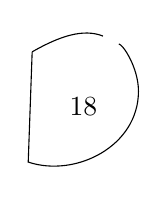
\begin{tikzpicture}[x=1mm,y=1mm]
\node at (0,0) {\mspage{18}};
\draw (-6.5,7)--(-7,-7) .. controls (-1,-9) and (7,-5) .. (7,2) .. controls (7,5) and (5,8) .. (4.5,8);
\draw (-6.5,7) .. controls (-3,9) and (0,10) .. (2.5,9);
\end{tikzpicture}}
% archive foliation: 89
\uuline{Dictionnaire}\qquad Fonctions $L$ --- \unsure{Cohomologie} à
\hfill action galoisienne.

Soit $k$ un \deleted{corps} anneau

\deleted{$\unsure{\mathcal A|\mathbf N}$ la catégorie}
\deleted{$\operatorname{Mod}(\mathbf Z)$ la catégorie}
$C$ la catégorie des modules de longueur
finie sur $k[t]=$ \deleted{vectoriels}\inserted{modules} $V$ \inserted{proj.}
de \deleted{dim}\inserted{rang} finie sur
$k$ munis d'un endomorphisme $f=$
$k[\unsure{\mathbf N|\mathbf Z}]$-modules, de \deleted{\unsure{rang}}\inserted{projectifs} finie sur $\unsure{\forall k|k}$.

Cette catégorie donne lieu à un faux-anneau,
noté $R^\bullet(\unsure{\mathbf N|\mathbf Z};k)$, qui est aussi, \inserted{si $k$ est un corps,}
le \deleted{\unsure{faux-anneau}} \inserted{groupe}
libre engendré par les classes des $k[\unsure{\mathbf N|\mathbf Z}]$-
modules simples, \inserted{finis sur $k$} or on connaît les $k[t]$-modules
simples, ce sont les polynômes \inserted{unitaires} irréductibles
$P\in k[t]$, en associant à $P$ le module
$k[t]/Pk[t]$. À tout tel $P$, \inserted{est} associé \unsure{à}
un $(V,f)$, dont le polynôme car. est
précisément $P$,
\margin{$k$ un corps ou non}
\[
P(t)=\det(t\,\mathrm{id}-f)
\]
[vrai pour $\forall P$, irréd. ou non !]. Il nous sera
plus commode de remplacer $P(t)$ par
\[
Q(t)=t^dP\left(\frac1t\right)=\det(1-tf)
\]
qui est un polynôme quelconque à coeff. cst égal $1$.
